\subsection{Жизнь без переменных}

\begin{frame}{Haskell}
	\begin{itemize}
		\item Haskell "--- чистый функциональный язык программирования.
		\item Компилируемый, статически типизирован, \textit{очень} мощная система типов.
		\item Есть огромное число библиотек.
		\item Очень чистый по сравнению с остальными языками вроде OCaml.
		\item Помимо функциональной чистоты имеет огромное количество интересных особенностей.
		\item На нём действительно можно писать код.
		\item Стандартный компилятор "--- GHC (Glasgow Haskell Compiler).
		\item Рекомендуется использовать в составе \href{https://www.haskell.org/platform/}{Haskell Platform}.
	\end{itemize}
\end{frame}

\begin{frame}{Демонстрация}
	\begin{enumerate}
		\item Демо: арифметика, простые типы, сравнения, списки, работа со списками, list comprehension.
		% 01-01-demo.hsi
		\item Упражнение: как найти все Пифагоровы тройки ($x^2 + y^2 = z^2$) при $1 \le x, y, z \le 10$?
		\item Интерпретатор \t{ghci} не поддерживает многострочные определения функций.
		\item Поэтому с некоторого момента лучше набирать код в файле, подгружая его в интерпретатор:
			\begin{itemize}
				\item \t{:load file.hs} (\t{:l file.hs}) компилирует \t{file.hs} и подгружает определения в интерпретатор.
				\item \t{:reload} перекомпилирует и переподключит все файлы.
			\end{itemize}
		\item Демо: функции, комментарии, определения функций <<и>>, <<или>>, <<сумма двух чисел>>.
		% 01-02-funcs.hs
	\end{enumerate}
\end{frame}

\begin{frame}{Жизнь без циклов}
	Упражнения на Python:
	\begin{itemize}
		\item Как посчитать сумму чисел в списке, если нет переменных и циклов?\pause
		\item Функция \t{sum}.\pause
		\item Как посчитать сумму квадратов чисел? \pause
		\item Определить лямбда-функцию для возведения в квадрат и применить \t{map} с \t{sum}.\pause
		\item Какие вообще операции со списками мы ещё не умеем делать без циклов? \pause
		\item В которых элементы влияют друг на друга.
	\end{itemize}
	Демо: то же самое на Haskell.
	% 01-03-exercise.hs
\end{frame}

\begin{frame}[fragile]{Не самый хороший императивный код}
	% 01-04-avg-len-imp.py
\begin{minted}{python}
s = "hello good world"
a = 0
b = 0
flag = False
for c in s + " ":
    if c == " ":
        if flag:
            a += 1
        flag = False
    else:
        b += 1
        flag = True
print(b / a)
\end{minted}
	И что тут происходит?
\end{frame}

\begin{frame}{Моя реакция на такой код}
	\begin{center}
		
\includegraphics{wtf-panda.png}
	\end{center}
\end{frame}

\begin{frame}[fragile]{На самом деле}
	Это вычисление средней длины слова в строке.

	Чем плохо?
	\begin{itemize}
		\item 11 строк на такое простое действие.
		\item Есть сложный инвариант.
		\item Тестировать сложно: надо подбирать специальную строку, на которой отличается средняя длина слов (а не просто воспроизводится баг).
	\end{itemize}
\end{frame}

\begin{frame}{Функциональное решение}
	\begin{itemize}
		\item Как записать то же самое функционально на Python? \pause
		\item Предполагаем, что есть функции \t{avg}, \t{map}, \t{split}. \pause
		\item \t{avg(map(len, "hello world".split()))} \pause
		% 01-05-avg-len-func.py
		\item Тут что-то сложное делает только функция split.
		\item Обычно \t{split()} пишут <<императивно>>, а всю последующую обработку "--- <<функционально>>.
		\item Таким образом императивная сложность изолирована, все кусочки можно тестировать по отдельности.
		\item Опять ввели абстракцию: три встроенные функции.
		\item Оказывается, что <<необходимых кирпичиков>> не так много.
	\end{itemize}
\end{frame}

\begin{frame}{Моя реакция на функциональный код}
	\begin{center}
		
\includegraphics[scale=0.3]{satisfied-seal.jpg}
	\end{center}
\end{frame}

\begin{frame}{Рандом в функциональном стиле}
	\begin{center}
		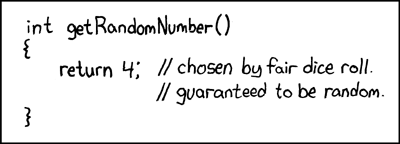
\includegraphics[scale=0.3]{random_number.png}
	\end{center}
\end{frame}
